%%==================================================================%%
%% Author : Abascal Fernández, Patricia                             %%
%%          Sánchez Barreiro, Pablo                                 %%
%% Version: 1.0, 16/04/2013                                         %%
%%                                                                  %%
%% Memoria del Proyecto Fin de Carrera                              %%
%% Background/Generación de Código con Epsilon                      %%
%===================================================================%%
Epsilon~\cite{kolovos:2008} es una plataforma para la construcción de lenguajes consistentes e interoperables para las tareas de gestión de modelado tales como transformación de modelos, generación de código, comparación de modelos, técnicas merge, refactorización y validación. El presente proyecto se ha centrado en la generación de código y por tanto en los lenguajes \emph{Epsilon Generation Language} (EGL) y \emph{Epsilon Object Language}(EOL) proporcionados por Epsilon, que se analizan con más detalle en las siguiente secciones.

\paragraph{Epsilon Generation Language(EGL)} \ \\

EGL proporciona un lenguaje apropiado para las transformaciones modelo a texto (\emph{model-to-text-transformation}, abreviado M2T). EGL puede ser usado para transformar modelos en varios tipos de artefactos de carácter textual, incluyendo códigos ejecutables (por ejemplo Java), informes (por ejemplo en HTML), imágenes (por ejemplo usando DOT), especificaciones formales (por ejemplo el lenguaje Z), o incluso aplicaciones completas generadas con múltiples lenguajes (por ejemplo HTML, Javascript y CSS).

EGL es un generador de código basado en plantillas; es decir, que la parte programada se asemeja al contenido que se va a generar, proporcionan además diversas caracteríticas que simplicifan y dan soporte a la generación de texto desde modelos. La Figura~\ref{back:fig:epsilonEGL} muestra un ejemplo sencillo del modelo de entrada para un programa EGL, donde se pueden observar tres clases: Persona, Alumno y Profesor. Supongamos que se quiere obtener el nombre de las clases, para ello se debería generar un código similar al de la Figura~\ref{back:code:generacionClases} donde aparece un bucle (líneas 1-3) que recorre todas las clases contenidas en el modelo de entrada y en cada una de ellas (línea 2) se genera el texto "El modelo contiene la clase: <nombre de la clase>". De esta forma, el resultado para el ejemplo de la Figura~\ref{back:fig:epsilonEGL} después de haber sido tratado mediante EGL tal como muestra la Figura~\ref{back:code:generacionClases} queda expuesto en la Figura~\ref{back:code:resultadogeneracionClases}.

\begin{figure}[!tb]
  \centering
	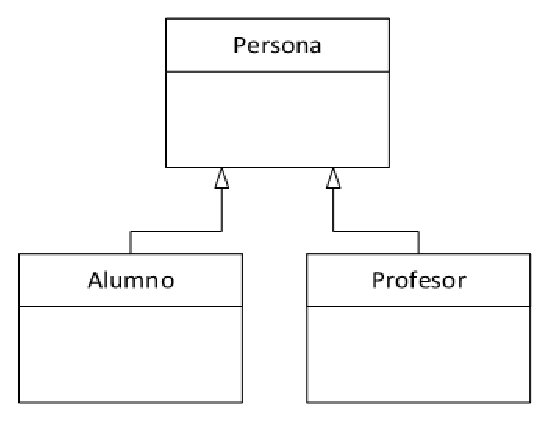
\includegraphics[width=.95\linewidth]{background/images/epsilonEGL.eps} \\
  \caption{Ejemplo de modelo de entrada para generación de código con EGL}
  \label{back:fig:epsilonEGL}
\end{figure}

\begin{figure}[tb!]
\begin{center}
\begin{footnotesize}
\begin{verbatim}
1 [% for (c in Class.all) { %]
2 El modelo contiene la clase: [%=c.name%]
3 [% } %]
\end{verbatim}
\end{footnotesize}
\end{center}
\caption{Generación del nombre de cada Class contenida en un modelo de entrada}
\label{back:code:generacionClases}
\end{figure}

\begin{figure}[tb!]
\begin{center}
\begin{footnotesize}
\begin{verbatim}
1 El modelo contiene la clase: Persona
2 El modelo contiene la clase: Alumno
3 El modelo contiene la clase: Profesor
\end{verbatim}
\end{footnotesize}
\end{center}
\caption{Resultado de la generación del nombre de cada Class contenida en un modelo de entrada}
\label{back:code:resultadogeneracionClases}
\end{figure}

 EGL no solo nos permite generar estos sencillos ejemplos, es una herramienta mucho más potente que permite la generación de funciones creadas específicamente por el usuario para facilitar la obtención de datos de los modelos de entrada. Tal como se aprecia en la Figura~\ref{back:code:generacionOperacion} se puede programar una operación que implemente la cabecera de una clase Java y de esta forma invocar dicha función tantas veces como sea necesario en aquellos programas EGL que lo necesiten. En la Figura~\ref{back:code:generacionOperacion} (línea 4) la operación \emph{visibility} indica la visibilidad de \emph{self} siendo en este caso la visibilidad de la clase tal como muestra la línea 3; mientras que la operación \emph{name} al igual que en la Figura~\ref{back:code:generacionClases} se refiere al nombre del elemento actual, en este caso el nombre de la clase.

\begin{figure}[tb!]
\begin{center}
\begin{footnotesize}
\begin{verbatim}
1 [%=c.declaration()%]
2 [% @template
3 operation Class declaration() { %]
4 [%=self.visibility] class [%=self.name%] {}
5 [% } %]
\end{verbatim}
\end{footnotesize}
\end{center}
\caption{Uso de una operación que especifica el texto generado para una declaración de una clase Java}
\label{back:code:generacionOperacion}
\end{figure}

El tipo Template proporciona tres utilidades básicas al usuario:

\begin{enumerate}
	\item  Una Template puede invocar a otras Templates y por tanto pueden ser compartidas y reutilizadas entre programas EGL. En la Figura~\ref{back:code:template} (línea 2) se aprecia cómo desde un programa EGL se llama a otro programa EGL.
    \item El tipo Template permite al usuario definir el destino del texto generado (por ejemplo a una base de datos o ficheros para un proyecto en Visual Studio).  En la Figura~\ref{back:code:template} (línea 3) se presenta que el fichero de salida será un fichero de extensión .txt.
    \item Y por último, proporciona un conjunto de operaciones que se usan para controlar el destino del texto generado. En la Figura~\ref{back:code:template} (línea 3) se muestra cómo se elige el fichero destino para almacenar el texto generado con la plantilla "ClassNames.egl".
\end{enumerate}

\begin{figure}[tb!]
\begin{center}
\begin{footnotesize}
\begin{verbatim}
1 [%
2 var t : Template = TemplateFactory.load("ClassNames.egl");
3 t.generate("Output.txt");
4 %]
\end{verbatim}
\end{footnotesize}
\end{center}
\caption{Almacenar el nombre de cada Class en disco}
\label{back:code:template}
\end{figure}


\paragraph{Epsilon Object Language(EOL)} \ \\

El principal objetivo de EOL es proporcionar un conjunto rehusable operaciones que son comunes en la gestión de modelos. La Figura~\ref{back:code:eol} muestra un ejemplo de operaciones EOL. No es un lenguaje orientado a objetos en el sentido de que no define clases de sí mismo pero sin embargo necesita gestionar objetos de los tipos definidos externamente a el (Figura~\ref{back:code:eol} líneas 3 y 7, en este caso objetos de tipo Integer). La línea 1 de la Figura~\ref{back:code:eol} presenta un ejemplo de llamada a operaciones EOL, donde el primer elemento es un 1, de tipo Integer, que llama a la operación add1() y devuelve, tal como se aprecia en la línea 4, el valor de \emph{self}+1 es decir 2. A continuación, se vuelve a tomar el valor 2, de tipo Integer, y se realiza la llamada a la operación add2() que devuelve el valor de \emph{self}+2 es decir 4. Y dicho contenido se imprime por pantalla (instrucción \emph{println()}).

\begin{figure}[tb!]
\begin{center}
\begin{footnotesize}
\begin{verbatim}
1 1.add1().add2().println();
2
3 operation Integer add1() : Integer {
4   return self + 1;
5 }
6
7 operation Integer add2() : Integer {
8   return self + 2;
9 } 
\end{verbatim}
\end{footnotesize}
\end{center}
\caption{Ejemplo de operación EOL}
\label{back:code:eol}
\end{figure}

De esta forma, EOL permite encapsular aquellas operaciones EGL que se vayan a utilizar a lo largo de las respectivas plantillas para evitar la repetición innecesaria de código.